\subsection{Login} \label{sec:Login}
Dette afsnit indeholder en gennemgang af grafisk brugergrænseflade, design og implementering af Login viewet i Rambøll Tilsyn.

\subsubsection{Design}
På figur \ref{fig:LoginSekvens} ses sekvens diagrammet for 'Login' viewet til Rambøll Tilsyn.
\begin{figure}[H] % (alternativt [H])
	\centering
	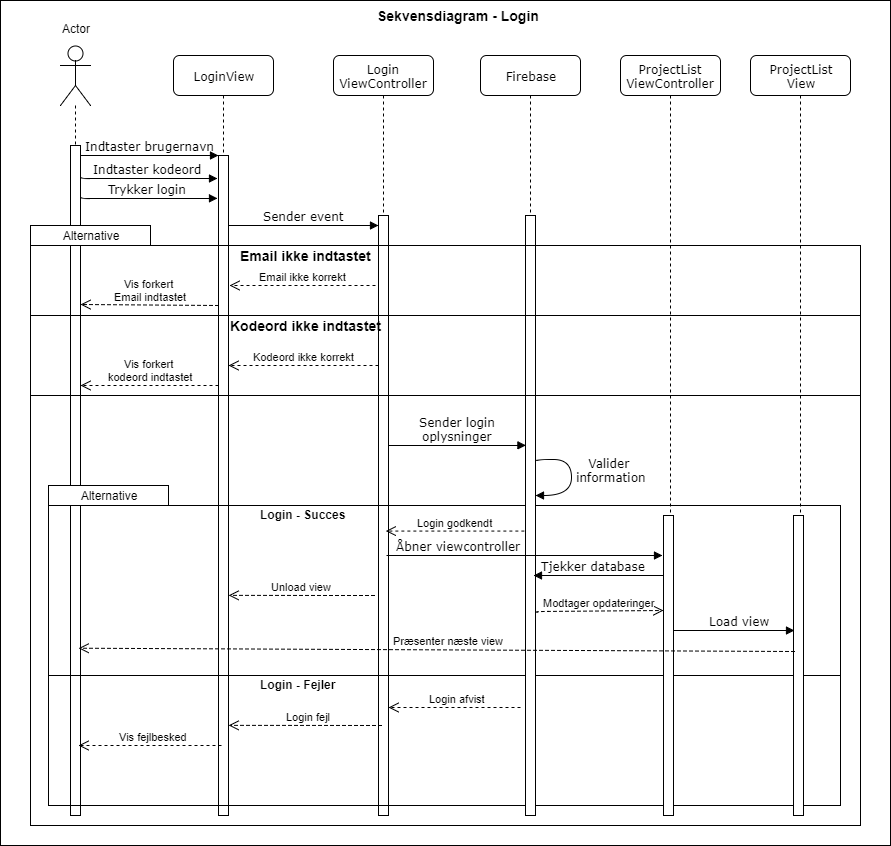
\includegraphics[height=15cm, width=15cm]{../ArkitekturDesign/Design/Login/LoginSekvensDiagram}
	\caption{Sekvensdiagram for Login i Rambøll Tilsyn.}
	\label{fig:LoginSekvens}
\end{figure}

\clearpage

\subsubsection{Grafisk brugergrænseflade}
I LoginViewet er der lavet felter til at bruger indtaster sit brugernavn og kodeord. Se figur \ref{fig:OpretBrugerView}
\begin{figure}[H] % (alternativt [H])
	\centering
	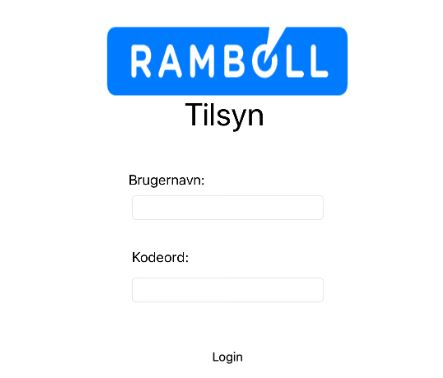
\includegraphics[height=12cm, width=10cm]{../ArkitekturDesign/Design/Login/LoginView}
	\caption{Login viewet som det er implementeret i Rambøll Tilsyn.}
	\label{fig:LoginView}
\end{figure}

\clearpage

\subsubsection{Implementering}
I dette afsnit vil der blive beskrevet funktionaliteten for de vigtigste funktioner i koden tilhørende 'Login' viewet.

På figur \ref{fig:Checkifusersigned}, ses funktionen for CheckIfUserSignedIn.
\begin{figure}[H] % (alternativt [H])
	\centering
	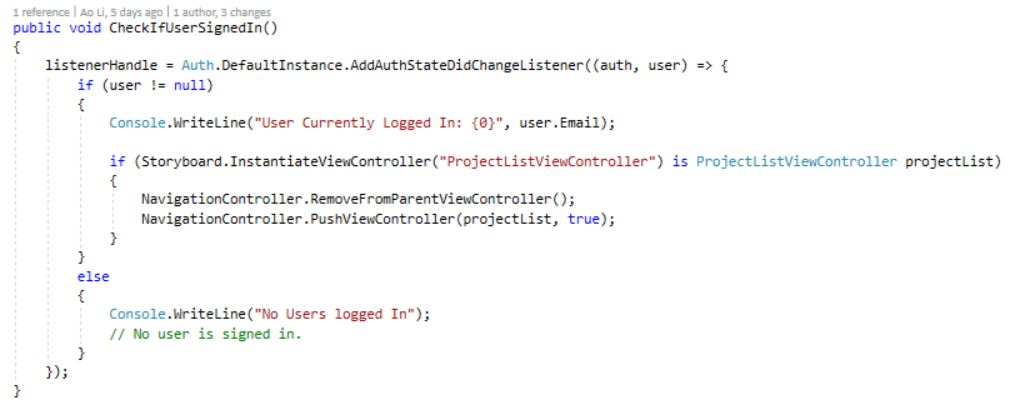
\includegraphics[height=8cm, width=15cm]{../ArkitekturDesign/Design/Login/Checkifusersigned}
	\caption{}
	\label{fig:Checkifusersigned}
\end{figure}
Først tjekker funktionen Firebases default instance, og ser om der er en bruger som er logget ind. \\
Er der en bruger logget ind, hoppes log ind over, og projekt listen bliver vist. \\
Ellers udskriver den at ingen bruger er logget ind.

På figur \ref{fig:ViewDidLoad}, ses funktionen for ViewDidLoad.
\begin{figure}[H] % (alternativt [H])
	\centering
	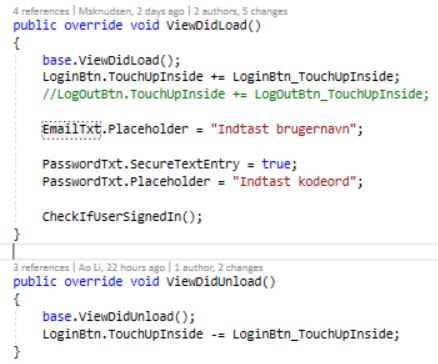
\includegraphics[height=7cm, width=12cm]{../ArkitekturDesign/Design/Login/ViewDidLoad}
	\caption{}
	\label{fig:ViewDidLoad}
\end{figure}

\clearpage

I ViewDidLoad, delegeres en eventhandler til LoginBtn.TouchUpInside. \\
Den indsætter placeholders i tekstfelterne Email og kodeord. Derudover maskere den inputs i kodeords tekstfeltet.
I ViewDidUnload fjernes eventhandleren fra LoginBtn.TouchUpInside, fordi at hvis dette ikke gøres, kan der opstå memory leak. \\

På figur \ref{fig:LoginBtn}, ses funktionen for LoginBtn.
\begin{figure}[H] % (alternativt [H])
	\centering
	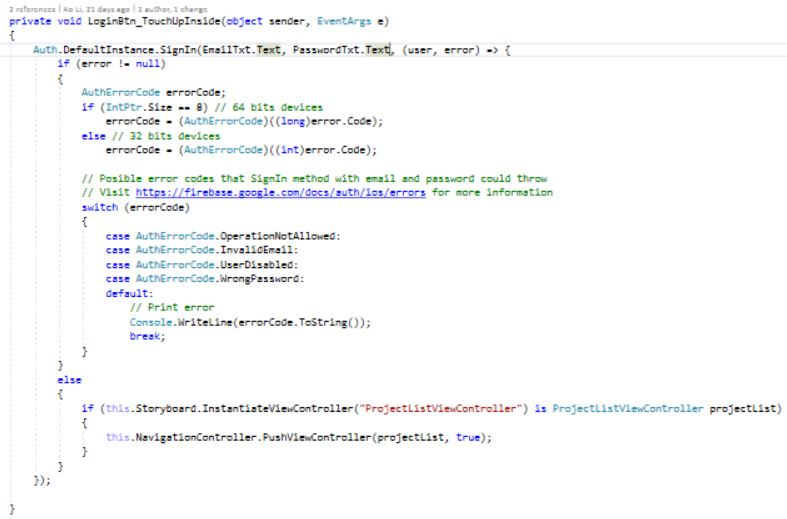
\includegraphics[height=10cm, width=18cm]{../ArkitekturDesign/Design/Login/LoginBtn}
	\caption{}
	\label{fig:LoginBtn}
\end{figure}
Tager default instance af Firebase Auth, kalder så SignIn metoden for denne instance og indsætter de to parametere skrevet i log ind viewet. \\
Efterfølgende valideres resultatet af log ind forsøget. Hvis der ingen fejl er, altså at email og kodeord er korrekt, så vil projekt listen blive vist. \\
Der kan i switch casen implementeres fejlhåndtering af diverse fejlkoder. 


\clearpage